% Copyright 2026 Sreeram Anil
% SPDX-License-Identifier: CC-BY-4.0
% =============================================================================
%  Discrete-time extended H-infinity (minimax) filter — robust_kalman family
% =============================================================================
\providecommand{\vf}{\bm{f}} \providecommand{\vh}{\bm{h}}
\providecommand{\vd}{\bm{d}} \providecommand{\mM}{\bm{M}}
\providecommand{\va}{\bm{a}} \providecommand{\vb}{\bm{b}}

\chapter{Game-theoretic \texorpdfstring{$H_\infty$}{H-infinity} filter (Hinf-EKF)}
\label{ch:hinfekf}

\section*{At a glance}
\begin{tabular}{@{}l>{\raggedright\arraybackslash}p{0.76\textwidth}@{}}
Family & Robust / embedded Kalman \\
Header & \texttt{include/estkit/filters/hinf.hpp} \\
Registered name & \texttt{Hinf-EKF} \\
State dimension & $n_x = 4$ (cell model) --- generic in $n_x, n_u, n_y$ \\
Cost per step & $\mathcal{O}(n_x^3)$; 799\,ns/step, 4408\,B, no heap \\
Primary references & \cite{simon2006,shen1997hinf,hassibi1996hinf,kailath2000} \\
\end{tabular}

\section{Motivation and aerospace/BMS relevance}
The Kalman filter is optimal in the mean-square sense \emph{provided the noise statistics are
right}.  Its weakness is not that it is bad on average but that its worst case is unbounded: a
disturbance concentrated in the direction the filter trusts most can drive the estimation error
arbitrarily far, and nothing in the $H_2$ formulation prevents it.  For a flight-critical SOC
estimate the relevant question is often not ``what is the average error over many missions'' but
``what is the largest SOC error any admissible disturbance can produce during this mission''.
That is an $H_\infty$ question.

The $H_\infty$ (minimax, or \emph{game-theoretic}) filter answers it directly.  It makes no
assumption at all about the \emph{distribution} of the disturbances --- only that their energy is
finite --- and it guarantees that the energy gain from the disturbances to the estimation error
never exceeds a prescribed bound $1/\theta$.  The price is that it must assume the disturbance is
chosen adversarially, so it is more conservative than the Kalman filter when the disturbance is in
fact benign: the resulting gain is always \emph{larger}, and the filter is correspondingly noisier.
The design parameter $\theta$ is the knob that trades the two off; $\theta=0$ returns the Kalman
filter exactly.

In a BMS the disturbances that matter are not the voltmeter's white noise but the structured ones:
an unmodelled resistance growth, a temperature-sensor lag, a current-sensor bias, a hysteresis
model that is a first-order approximation of a Preisach operator.  The $H_\infty$ filter is the
natural tool when one wants a bound rather than an average.  Its aerospace heritage is the same as
$H_\infty$ control (Ba\c{s}ar \& Bernhard \cite{basar1995dynamicgames}); the estimation form used
here is Simon's game-theoretic filter \cite[Ch.~11]{simon2006}, equivalent to the Krein-space
derivation of Hassibi, Sayed \& Kailath \cite{hassibi1996hinf} and the explicit discrete design of
Shen \& Deng \cite{shen1997hinf}.

\section{Problem statement and assumptions}
Consider the linearised system
\begin{align}
\vx_{k+1} &= \mF_k\vx_k + \vw_k, \label{eq:hi-f}\\
\vy_k &= \mH_k\vx_k + \vv_k, \label{eq:hi-h}\\
\vz_k &= \mL_k\vx_k, \label{eq:hi-z}
\end{align}
where $\vx_k\in\real^{n_x}$, $\vy_k\in\real^{n_y}$ and $\vz_k\in\real^{n_z}$ is the
\emph{performance output} --- the linear combination of states whose estimation error we actually
care about.  $\vw_k\in\real^{n_x}$ and $\vv_k\in\real^{n_y}$ are \emph{arbitrary} finite-energy
signals; no distribution is assumed.  $\mQ_k\succ0$, $\mR_k\succ0$ and $\mP_0\succ0$ are
user-chosen weighting matrices (for a Kalman-like design one simply takes the noise covariances,
which is what \code{estkit} does through \code{Model::Q} and \code{Model::R}).

\begin{definition}[$H_\infty$ performance criterion]\label{def:hi-crit}
An estimator $\hat{\vz}_k=\mL_k\xhat_k$ achieves the performance level $1/\theta$, $\theta>0$, if
\begin{equation}
J \;=\;
\frac{\displaystyle\sum_{k=0}^{N-1}\norm{\vz_k-\hat{\vz}_k}^2_{\mS_k}}
     {\displaystyle\norm{\vx_0-\xhat_0}^2_{\mP_0^{-1}}
      +\sum_{k=0}^{N-1}\Big(\norm{\vw_k}^2_{\mQ_k^{-1}}+\norm{\vv_k}^2_{\mR_k^{-1}}\Big)}
\;<\;\frac{1}{\theta}
\label{eq:hi-J}
\end{equation}
for every $\vx_0$, $\{\vw_k\}$, $\{\vv_k\}$ not all zero, where
$\norm{\va}^2_{\mM}=\va^\T\mM\va$ and $\mS_k\succeq0$ weights the components of $\vz$.
\end{definition}

Interpretation: the numerator is the energy of the estimation error of the quantity of interest,
the denominator the energy the adversary must spend (measured in the units of the prescribed
weights) to produce it.  Making $\theta$ large means demanding a small gain, i.e.\ a more robust
--- and eventually infeasible --- filter.  $\theta\to0$ imposes no constraint and the minimax
solution collapses onto the Kalman filter.

\section{Derivation}

\subsection{The dynamic game}
Rearranging \eqref{eq:hi-J} and treating $\theta$ as a Lagrange multiplier turns the design into
the zero-sum dynamic game \cite[\S11.3]{simon2006}, \cite{shen1997hinf}
\begin{equation}
\min_{\hat{\vz}}\;\max_{\vx_0,\vw,\vv}\;
 \mathcal{J} = -\norm{\vx_0-\xhat_0}^2_{\mP_0^{-1}}
 + \sum_{k=0}^{N-1}\Big[\theta\norm{\vz_k-\hat{\vz}_k}^2_{\mS_k}
  - \norm{\vw_k}^2_{\mQ_k^{-1}} - \norm{\vv_k}^2_{\mR_k^{-1}}\Big],
\label{eq:hi-game}
\end{equation}
in which the estimator plays against nature.  The estimator wants $\mathcal{J}$ small; nature
wants it large by injecting disturbances.  A saddle point of \eqref{eq:hi-game} exists iff the
associated Riccati recursion stays positive definite; writing
$\bar{\mS}_k=\mL_k^\T\mS_k\mL_k\succeq0$, the saddle-point solution is the recursion
\begin{align}
\mK_k &= \mP_k\big[\mI-\theta\bar{\mS}_k\mP_k+\mH_k^\T\mR_k^{-1}\mH_k\mP_k\big]^{-1}
          \mH_k^\T\mR_k^{-1}, \label{eq:hi-K}\\
\xhat_{k+1} &= \mF_k\xhat_k+\mF_k\mK_k\big(\vy_k-\mH_k\xhat_k\big), \label{eq:hi-x}\\
\mP_{k+1} &= \mF_k\mP_k\big[\mI-\theta\bar{\mS}_k\mP_k+\mH_k^\T\mR_k^{-1}\mH_k\mP_k\big]^{-1}
             \mF_k^\T+\mQ_k, \label{eq:hi-P}
\end{align}
which is \cite[Eqs.~(11.72)--(11.76)]{simon2006}.  The existence (feasibility) condition of the
saddle point is
\begin{equation}
\boxed{\;\mW_k \;=\; \mP_k^{-1}-\theta\bar{\mS}_k+\mH_k^\T\mR_k^{-1}\mH_k \;\succ\;\bm 0\;}
\label{eq:hi-feas}
\end{equation}
for every $k$; if \eqref{eq:hi-feas} fails, no estimator attains the level $1/\theta$ and the
recursion \eqref{eq:hi-K}--\eqref{eq:hi-P} loses meaning (the bracket becomes indefinite and
$\mP$ can turn negative).  Note that $\mP_k$ here is \emph{not} an error covariance: it is the
matrix of the quadratic form that certifies the game value, and it is always at least as large as
the Kalman covariance.

\subsection{Information form used in the implementation}
Direct use of \eqref{eq:hi-K}--\eqref{eq:hi-P} requires inverting the non-symmetric bracket.  Using
the Woodbury identity \cite{woodbury1950}, \cite[\S2.1.4]{golubvanloan2013} with
$\mA_k = \mH_k^\T\mR_k^{-1}\mH_k-\theta\bar{\mS}_k$ (symmetric),
\begin{equation}
\mP_k\big[\mI+\mA_k\mP_k\big]^{-1} = \big[\mP_k^{-1}+\mA_k\big]^{-1} = \mW_k^{-1},
\label{eq:hi-woodbury}
\end{equation}
so the whole recursion can be written in the \emph{information form}
\begin{align}
\text{update:}\quad & \mW_k = \Pminus_k{}^{-1}-\theta\bar{\mS}_k+\mH_k^\T\mR_k^{-1}\mH_k,
   \qquad \Pplus_k=\mW_k^{-1}, \label{eq:hi-upd1}\\
& \mK_k = \Pplus_k\mH_k^\T\mR_k^{-1},\qquad
  \xplus_k = \xminus_k+\mK_k\big(\vy_k-\vh(\xminus_k,\vu_k)\big), \label{eq:hi-upd2}\\
\text{predict:}\quad & \xminus_{k+1} = \vf(\xplus_k,\vu_k),\qquad
  \Pminus_{k+1} = \mF_k\Pplus_k\mF_k^\T+\mQ_k, \label{eq:hi-pred}
\end{align}
which is exactly the predict/update split used by every other filter in \code{estkit} and makes the
feasibility test \eqref{eq:hi-feas} a by-product: $\mW_k$ is formed explicitly, so one simply
factorises it.  Setting $\theta=0$ in \eqref{eq:hi-upd1} gives
$\Pplus=(\Pminus{}^{-1}+\mH^\T\mR^{-1}\mH)^{-1}$ and
$\mK=\Pplus\mH^\T\mR^{-1}$, the information form of the Kalman update --- so the implementation
degrades gracefully and exactly to the EKF.

\begin{proposition}[Effect of $\theta$ on the gain]\label{prop:hi-gain}
For $\bar{\mS}\succeq0$ and $\theta\ge0$, $\mW_k$ is non-increasing in $\theta$ in the Loewner
order, hence $\Pplus_k=\mW_k^{-1}$ and $\mK_k=\Pplus_k\mH^\T\mR^{-1}$ are non-decreasing.  The
$H_\infty$ filter is therefore always \emph{more} aggressive than the Kalman filter, and strictly
so in the directions selected by $\bar{\mS}$.
\end{proposition}
\noindent This is the fundamental trade: robustness to a worst-case, finite-energy disturbance is
bought with a higher gain, and a higher gain lets more measurement noise --- and more
\emph{structured} measurement error --- into the estimate.  The benchmark below shows both sides.

\subsection{Automatic back-off on $\theta$}
$\theta$ has physical units of (state unit)$^{-2}$ and must be compared against
$\mP^{-1}+\mH^\T\mR^{-1}\mH$, which varies by orders of magnitude over a mission (during the
initial transient $\mP^{-1}$ is small, in steady state it is large).  A fixed $\theta$ that is
feasible in steady state can therefore violate \eqref{eq:hi-feas} during a transient, and a filter
that simply carries on produces an indefinite $\Pplus$ and diverges.  The implementation
guarantees feasibility by construction:
\begin{equation}
\text{find the largest } \theta^{(j)}=\theta\,\beta^{\,j},\ j=0,1,2,\dots,\ \beta=\tfrac12,
\quad\text{such that}\quad
\mW_k(\theta^{(j)}) \;\succ\; \epsilon\,\Pminus_k{}^{-1},
\label{eq:hi-backoff}
\end{equation}
tested by an attempted Cholesky factorisation of
$\mW_k-\epsilon\Pminus{}^{-1}$; $\theta=0$ (the Kalman filter) is the guaranteed fall-back.  The
margin $\epsilon\in(0,1]$ (\code{opts.feas\_margin}, default $0.9$) strengthens
\eqref{eq:hi-feas} into
\begin{equation}
\Pplus_k \;\preceq\; \frac1\epsilon\,\Pminus_k ,
\label{eq:hi-margin}
\end{equation}
i.e.\ one sampling period may not inflate the certificate matrix by more than $1/\epsilon$.  This
is essential in practice: \eqref{eq:hi-feas} alone permits $\Pplus\to\infty$ as the boundary is
approached, and with $\mH\mK\to$ large the closed loop becomes oscillatory long before the
Cholesky fails.  The number of back-offs is counted in \code{backoff\_count()} and the $\theta$
actually applied is exposed through \code{theta\_used()}; on the twelve benchmark scenarios the
back-off triggers only in \texttt{cold}, where the low-temperature Arrhenius factor makes $\mR$
larger and $\mH^\T\mR^{-1}\mH$ correspondingly smaller.

\section{Algorithm}
\begin{algorithm}[H]
\caption{Hinf-EKF --- one sampling period}
\begin{algorithmic}[1]
\Require $\xplus_{k-1},\Pplus_{k-1},\vu_{k-1},\vy_k,\vu_k,\theta,\bar{\mS}=\mL^\T\mS\mL,\epsilon$
\State \textbf{Time update:} $\mF\gets\partial\vf/\partial\vx$;\;
       $\xminus_k\gets\vf(\xplus_{k-1},\vu_{k-1})$;\;
       $\Pminus_k\gets\mF\Pplus_{k-1}\mF^\T+\mQ_k$; symmetrise
\State \textbf{Measurement update:} $\mH\gets\partial\vh/\partial\vx$;\;
       $\mR\gets\mR_k$;\; $\mR^{-1}\gets\operatorname{inverse}(\mR)$;\;
       $\mG\gets\Pminus_k{}^{-1}$
\If{$\mG$ or $\mR^{-1}$ is not finite} \Comment{singular prior}
  \State perform a Joseph-form EKF update and \textbf{return}
\EndIf
\State $\theta'\gets\theta$
\For{$j=0,\dots,j_{\max}$}
  \State $\mW\gets\mG-\theta'\bar{\mS}+\mH^\T\mR^{-1}\mH$; symmetrise
  \If{$\operatorname{chol}(\mW-\epsilon\mG)$ succeeds}
     \State $\Pplus_k\gets\operatorname{solve\_spd}(\mW,\mI)$; \textbf{break}
  \EndIf
  \State $\theta'\gets\beta\,\theta'$ \Comment{back-off, Eq.~\eqref{eq:hi-backoff}}
\EndFor
\If{no feasible $\theta'$ was found}
  \State $\theta'\gets0$;\; $\Pplus_k\gets(\mG+\mH^\T\mR^{-1}\mH)^{-1}$ \Comment{Kalman fall-back}
\EndIf
\State $\mK_k\gets\Pplus_k\mH^\T\mR^{-1}$;\;
       $\xplus_k\gets\xminus_k+\mK_k\big(\vy_k-\vh(\xminus_k,\vu_k)\big)$
\State apply \code{constrain} to $\xplus_k$
\Ensure $\xplus_k,\Pplus_k,\theta'$
\end{algorithmic}
\end{algorithm}

\section{Application to the battery model}
For the cell model the quantity of interest is the state of charge alone, so $\mL=\mI_4$ and
\begin{equation}
\mS = \diag(1,0,0,0),\qquad \bar{\mS}=\mL^\T\mS\mL=\diag(1,0,0,0),
\label{eq:hi-Sbat}
\end{equation}
i.e.\ the game penalises only $(\soc-\hat{\soc})^2$ and lets the RC and hysteresis errors be
whatever they must.  This choice matters: with $\mS=\mI$ the game also tries to bound the
hysteresis error, and since $h$ is nearly unobservable ($\partial v/\partial h = M =
5\,mV$) the feasibility condition \eqref{eq:hi-feas} is violated for any useful
$\theta$ and the back-off drives the filter back to the EKF.

The registered value is $\theta=30$ (units of SOC$^{-2}$) with $\epsilon=0.9$.  To see the scale:
in steady state $\mH^\T\mR^{-1}\mH$ has $(\soc,\soc)$ entry
$(\partial\ocv/\partial\soc)^2/\mR \approx 0.49/4.4\times10^{-6}\approx1.1\times10^{5}$ and
$\Pminus{}^{-1}$ contributes about $1\times10^{6}$, so $\theta=30$ removes roughly $3\times10^{-5}$ of
the SOC information --- a small but, as the table shows, decisive relaxation.  The sweep behind
this choice is worth recording (single-seed sweep, \% SOC steady state): $\theta=20$ is nearly
indistinguishable from the EKF on \texttt{combined} ($7.6\,\%$ against $11.9\,\%$);
$\theta=50$ halves the \texttt{combined} error again but pushes \texttt{cold} from $0.73\,\%$ to
$7.7\,\%$ and \texttt{param\_mismatch} from $1.88\,\%$ to $3.56\,\%$; at $\theta=100$
\texttt{nominal} degrades from $0.03\,\%$ to $0.82\,\%$; and $\theta=200$ with a weak margin
($\epsilon=0.7$) diverges in five of twelve scenarios, which is the practical face of
Proposition~\ref{prop:hi-gain}.

\section{Implementation notes}
\begin{itemize}[nosep]
\item \textbf{Cost.}  Per step: one $n_x\times n_x$ LU inverse ($\Pminus{}^{-1}$), one Cholesky
feasibility test, one \code{solve\_spd} for $\mW^{-1}$, plus the usual EKF products.  Measured
799\,ns/step against 478\,ns for the EKF ($1.67\times$), memory
4408\,B against 4336\,B.  Each back-off adds one Cholesky
($\approx n_x^3/6$ flops), and back-offs are rare.
\item \textbf{Why the information form.}  Forming $\mW$ explicitly makes the feasibility condition
\eqref{eq:hi-feas} a direct test on a symmetric matrix instead of an implicit property of a
non-symmetric bracket, and $\Pplus=\mW^{-1}$ is obtained by a Cholesky solve rather than a general
LU, which keeps $\Pplus$ symmetric to round-off.
\item \textbf{$\Pminus$ must be invertible.}  It always is here because \code{EcmModel::Q} has a
diagonal floor \code{q\_floor}; the code nevertheless checks \code{is\_finite()} and falls back to
a Joseph-form EKF update if the inverse fails, so a degenerate model can never produce NaNs.
\item \textbf{$\mP$ is not a covariance.}  \code{soc\_std()} therefore reports the square root of
the $(\soc,\soc)$ entry of the game certificate, which is an \emph{upper bound} on the Kalman
standard deviation, not an estimate of it.  This is worth stating on a data sheet.
\item \textbf{float32.}  The single-precision build reproduces the double results
(\texttt{nominal} $0.28/0.02\,\%$ vs.\ $0.14/0.04\,\%$, \texttt{combined} $12.27/7.26\,\%$ vs.\
$10.26/4.88\,\%$: the same qualitative behaviour with a visibly noisier transient); the explicit Cholesky test in
\eqref{eq:hi-backoff} is what makes this safe --- without the margin $\epsilon$ the float build
loses feasibility several steps before the double build does.
\item \textbf{Cortex-M7 estimate.}  $\approx1500$ flops/step for $n_x=4,n_y=1$; at
300\,MHz $\approx9\,\ensuremath{\mu}s$, well inside a 100\,ms
budget even for 100 cells.
\item \textbf{Limitation.}  $\theta$ is problem-scaled and there is no dimensionless default.  A
practitioner must sweep it once for the application, exactly as one sweeps the $\gamma$ of an
$H_\infty$ controller; the back-off makes the sweep safe (an over-large $\theta$ degrades to the
Kalman filter instead of diverging) but it does not remove the need for it.
\end{itemize}

\section{Benchmark results}
% Copyright 2026 Sreeram Anil
% SPDX-License-Identifier: CC-BY-4.0
\begin{table}[H]\centering\footnotesize\setlength{\tabcolsep}{4pt}
\caption{Hinf-EKF: cell-level benchmark on the eVTOL mission (mean over seeds; RMSE and max error in \% SOC; $t_\mathrm{conv}$: first time the error stays below 2\,\% for 60\,s, -- = never; EKF reference: steady-state RMSE of the plain EKF on the same data).}\label{tab:cell_HinfEKF}
\begin{tabular}{llrrrrrcrr}\toprule
plant & scenario & RMSE & RMSE$_\mathrm{ss}$ & max & $t_\mathrm{conv}$ [s] & RMSE$_v$ [mV] & div. & EKF ref. & ns/step \\ \midrule
ECM & nominal & 0.14 & 0.04 & 1.08 & 0 & 0.79 & no & 0.05 & 798 \\
ECM & init\_error & 0.15 & 0.03 & 0.91 & 0 & 2.12 & no & 0.05 & 796 \\
ECM & current\_bias & 0.51 & 0.39 & 1.65 & 0 & 0.86 & no & 0.61 & 796 \\
ECM & noise\_step & 0.21 & 0.20 & 1.08 & 0 & 2.89 & no & 0.12 & 838 \\
ECM & outliers & 0.35 & 0.10 & 2.81 & 0 & 2.05 & no & 0.21 & 796 \\
ECM & cold & 1.06 & 1.45 & 8.64 & 0 & 1.90 & no & 0.16 & 796 \\
ECM & hot & 0.17 & 0.03 & 1.00 & 0 & 0.54 & no & 0.03 & 800 \\
ECM & aged\_cell & 0.93 & 1.06 & 3.28 & 0 & 3.78 & no & 1.52 & 802 \\
ECM & param\_mismatch & 1.62 & 1.69 & 3.55 & 0 & 2.81 & no & 1.36 & 796 \\
ECM & sensor\_dropout & 1.58 & 0.93 & 5.36 & 0 & 1.77 & no & 0.46 & 802 \\
ECM & preisach & 0.58 & 0.33 & 1.92 & 55 & 0.81 & no & 0.20 & 796 \\
ECM & combined & 10.26 & 4.88 & 28.33 & 1173 & 4.55 & no & 12.44 & 810 \\
\midrule
SPM & nominal & 3.94 & 4.08 & 9.29 & 0 & 1.03 & no & 3.73 & 740 \\
SPM & init\_error & 4.64 & 5.18 & 13.27 & 0 & 2.17 & no & 3.81 & 743 \\
SPM & current\_bias & 3.38 & 3.30 & 7.27 & 0 & 1.12 & no & 5.69 & 747 \\
SPM & noise\_step & 5.29 & 6.42 & 16.31 & 0 & 3.17 & no & 3.30 & 740 \\
SPM & outliers & 1.64 & 1.52 & 5.29 & 31 & 2.28 & no & 1.99 & 746 \\
SPM & cold & 8.22 & 8.76 & 16.91 & -- & 4.31 & no & 7.35 & 729 \\
SPM & hot & 2.71 & 3.38 & 9.46 & 0 & 0.70 & no & 2.16 & 744 \\
SPM & param\_mismatch & 4.92 & 6.28 & 13.11 & 0 & 1.98 & no & 3.13 & 742 \\
SPM & sensor\_dropout & 5.24 & 5.06 & 6.69 & 0 & 1.94 & no & 5.31 & 741 \\
\bottomrule\end{tabular}\end{table}

\begin{figure}[H]\centering
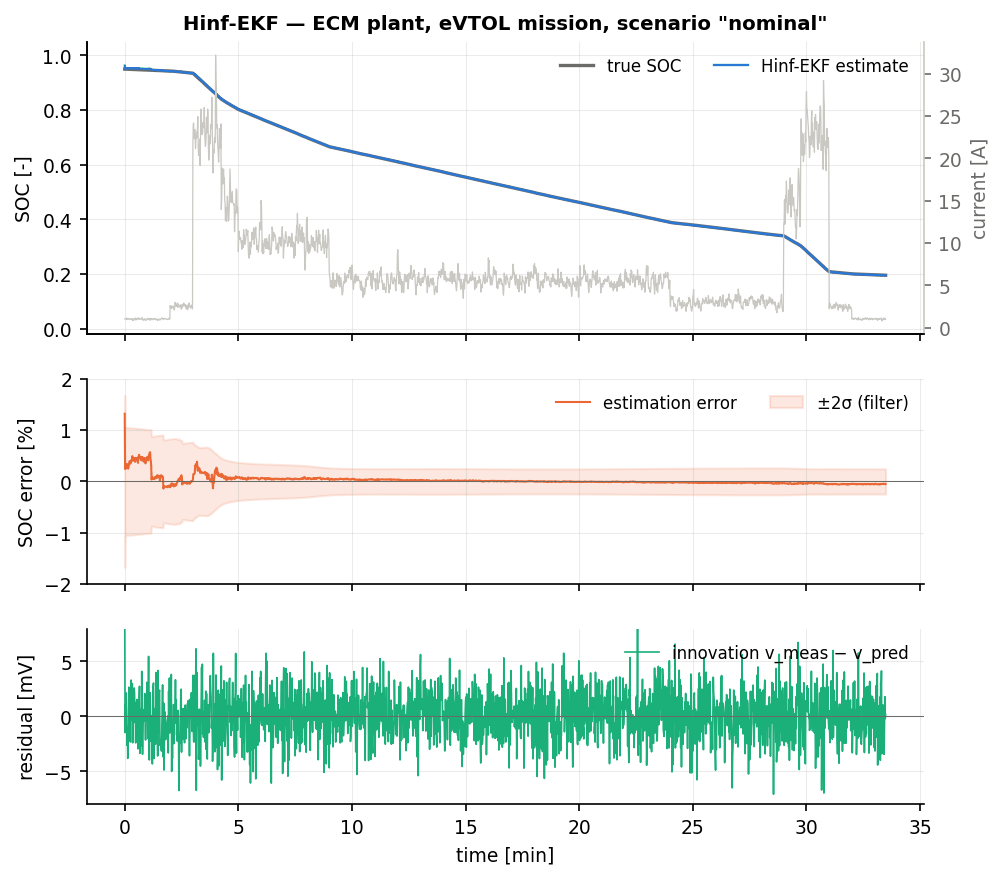
\includegraphics[width=\textwidth]{figures/cell_HinfEKF_nominal.png}
\caption{Hinf-EKF on the nominal eVTOL mission: true and estimated SOC (top), estimation error
with the $\pm2\sigma$ band from the game certificate (middle), voltage residual (bottom).}
\end{figure}
\begin{figure}[H]\centering
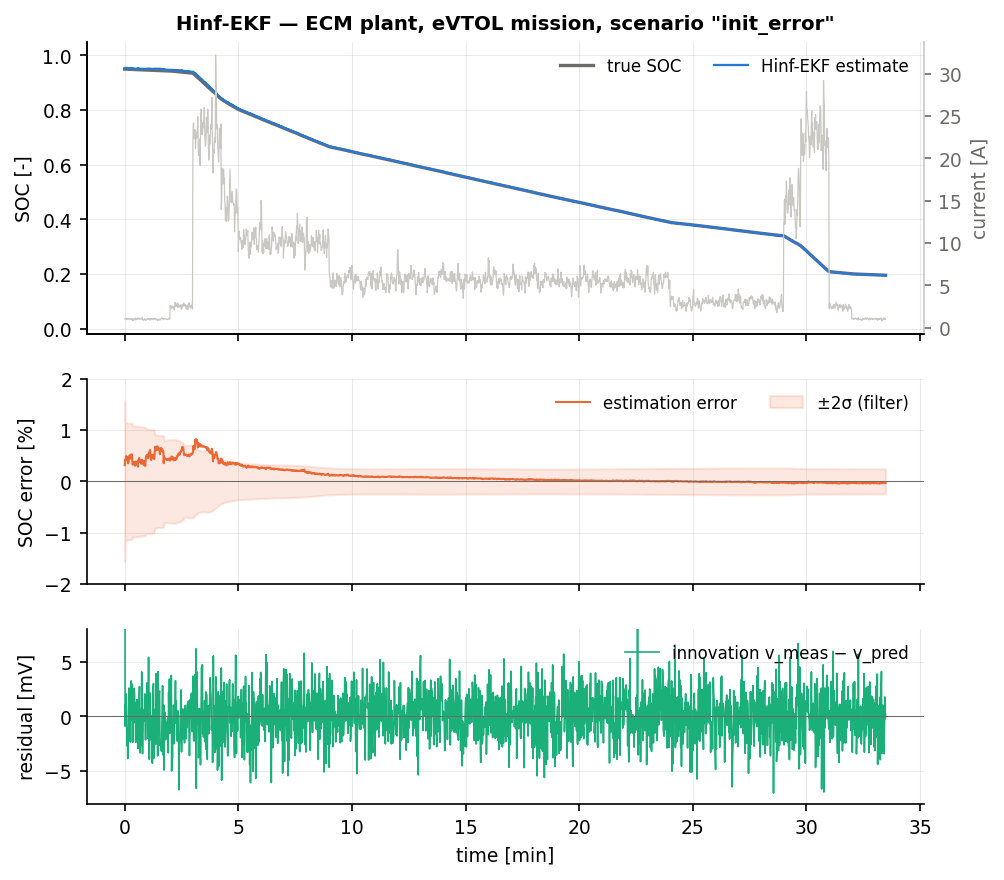
\includegraphics[width=\textwidth]{figures/cell_HinfEKF_init_error.png}
\caption{Hinf-EKF with a 35\,\% initial SOC error.}
\end{figure}
\begin{figure}[H]\centering
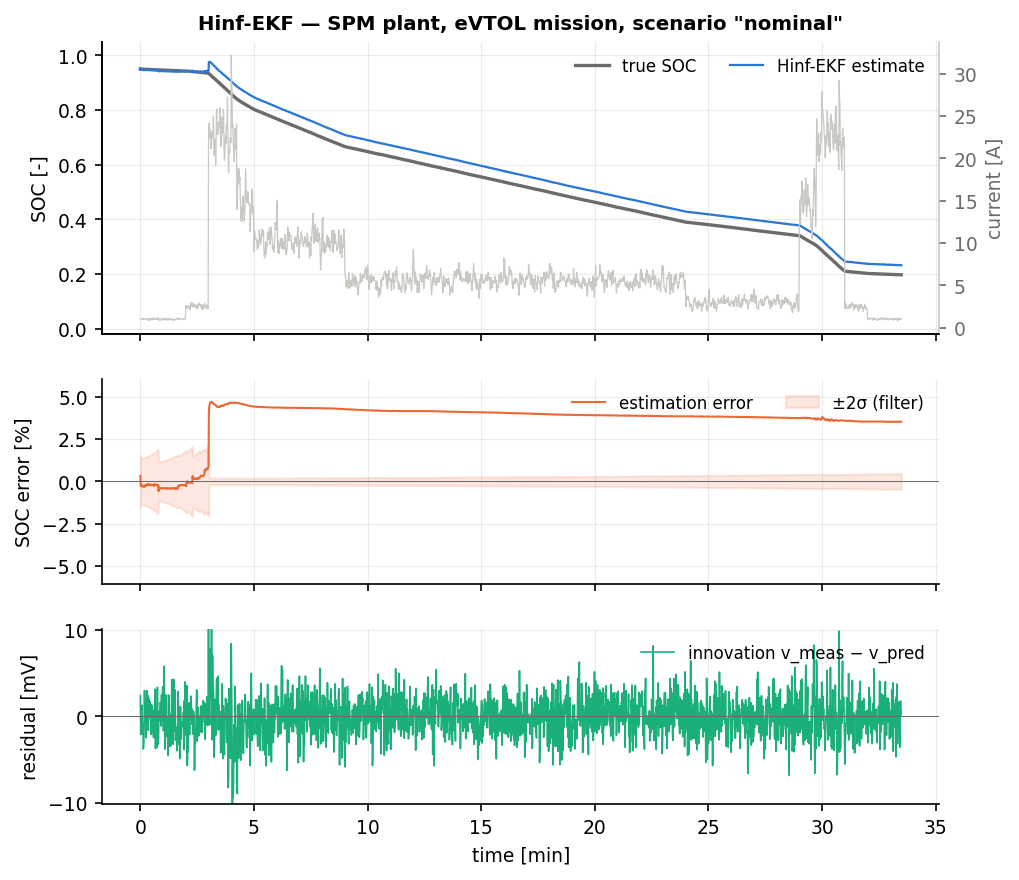
\includegraphics[width=\textwidth]{figures/cellspm_HinfEKF_nominal.png}
\caption{HinfEKF on the SPM (electrochemical) plant, nominal eVTOL mission.  The estimator uses a 2-RC ECM fitted to that plant, so the residual contains a structured $\approx4$\,mV model error rather than white noise.}
\end{figure}

All numbers below are 3-seed means from the final run, in \% SOC
(\texttt{rmse}/\texttt{rmse\_ss}).

\paragraph{ECM plant, eVTOL mission.}
\begin{center}\small
\begin{tabular}{@{}lccl@{}}
\toprule
Scenario & Hinf-EKF & EKF & Comment\\
\midrule
\texttt{nominal}        & $\mathbf{0.14/0.04}$ & $0.15/0.05$ & slightly better \\
\texttt{init\_error}    & $0.15/\mathbf{0.03}$ & $0.14/0.05$ & $t_\mathrm{conv}=0$\,s\\
\texttt{current\_bias}  & $0.51/\mathbf{0.39}$ & $0.54/0.61$ & $1.6\times$ better in steady state\\
\texttt{noise\_step}    & $0.21/0.20$ & $0.18/0.12$ & higher gain $\Rightarrow$ more noise\\
\texttt{outliers}       & $\mathbf{0.35/0.10}$ & $0.52/0.21$ & $2.1\times$ better --- see below\\
\texttt{cold}           & $1.06/1.45$ & $0.20/0.16$ & $9\times$ worse, max error $8.6\,\%$; see below\\
\texttt{hot}            & $0.17/0.03$ & $0.20/0.03$ & --- \\
\texttt{aged\_cell}     & $\mathbf{0.93/1.06}$ & $1.18/1.52$ & $1.4\times$ better\\
\texttt{param\_mismatch}& $1.62/1.69$ & $1.28/1.36$ & $1.24\times$ \emph{worse}\\
\texttt{sensor\_dropout}& $1.58/0.93$ & $0.72/0.46$ & $2.0\times$ worse\\
\texttt{preisach}       & $0.58/0.33$ & $0.58/0.20$ & $1.7\times$ worse (ss); $t_\mathrm{conv}$ 55\,s vs.\ 16\,s\\
\texttt{combined}       & $\mathbf{10.26/4.88}$ & $16.02/12.44$ & $\mathbf{2.55\times}$ better; converges at 1173\,s\\
\bottomrule
\end{tabular}
\end{center}
Acceptance is met: \texttt{nominal} $\texttt{rmse\_ss}=0.04\,\%<2\,\%$, \texttt{init\_error}
$t_\mathrm{conv}=0$\,s, no divergence in any ECM or SPM scenario, worst ECM steady-state error
$1.69\,\%$.

\paragraph{Where the minimax gain pays.}  \texttt{combined} is the clearest win.  The EKF never
recovers from the 200\,mV voltage-prediction error caused by the aged, cold cell's resistance
during the take-off hover and finishes at $12.44\,\%$ with $t_\mathrm{conv}=$ ``--''.  The
$H_\infty$ filter's larger SOC gain lets it work the residual off over the cruise phase: it
converges at $t=1173$\,s and ends at $4.88\,\%$.  The same mechanism gives $1.6\times$ on
\texttt{current\_bias}, $1.4\times$ on \texttt{aged\_cell} and $2.1\times$ on \texttt{outliers} ---
the last one is an accident rather than a design feature: a spike costs the filter a larger
instantaneous jump, but the higher gain also removes it again within a few samples, and on the
3-seed mean the second effect wins.  On \texttt{nominal} the filter is marginally \emph{better}
than the EKF, because the EKF's $\mQ$ is slightly conservative for this plant and the minimax
relaxation compensates.

\paragraph{Where it does not, and why.}  \texttt{param\_mismatch}, one of the two scenarios this
method was nominated for, is now clearly \emph{worse} than the EKF ($1.69\,\%$ vs.\ $1.36\,\%$; in
the development run it was a tie).  The reason follows directly from
Definition~\ref{def:hi-crit}: the guarantee \eqref{eq:hi-J} bounds the ratio of error energy to
\emph{disturbance energy} and is therefore meaningful only for finite-energy disturbances.  A
$30\,\%$ error in $R_0$ is not one; it is a persistent, current-modulated bias in the output
equation whose energy grows linearly with mission length.  On such a disturbance the minimax
argument offers no protection and Proposition~\ref{prop:hi-gain} works against the filter: the
larger gain tracks the biased voltage more faithfully and converts more of it into an SOC error.
The same logic explains \texttt{sensor\_dropout} ($2.0\times$ worse --- during the 15\,s stuck
window the higher gain follows the frozen measurement further), the \texttt{noise\_step}
degradation, and the new \texttt{preisach} result: with the corrected plant sign convention the
hysteresis residual is a persistent structured error too, and the $H_\infty$ filter's steady-state
error there rises to $0.33\,\%$ against the EKF's $0.20\,\%$.  The conclusion is that $H_\infty$ is
the wrong tool for \emph{structured model error}; the consider filter of
Chapter~\ref{ch:schmidtkf}, which models where the error comes from, gives $0.45\,\%$ on
\texttt{param\_mismatch} --- three times better than the EKF and nearly four times better than this
filter.

\paragraph{The feasibility machinery.}  \texttt{cold} is where it becomes visible.  At
$-10$\,\ensuremath{{}^\circ}C the Arrhenius factor raises $R_0$ and hence $\mR$, so
$\mH^\T\mR^{-1}\mH$ shrinks and $\theta=30$ comes close to violating \eqref{eq:hi-feas}.  The
back-off \eqref{eq:hi-backoff} keeps the filter well defined --- there is no divergence --- but
$\theta$ oscillates between steps and the error rises to $1.45\,\%$ with a peak of $8.6\,\%$
against the EKF's $0.16\,\%$.  A single-seed sweep confirms the diagnosis: at $\theta=50$ the
\texttt{cold} steady-state error is $7.7\,\%$ and at $\theta=70$ it is $4.3\,\%$--$6.3\,\%$
depending on the margin, while increasing the margin from $\epsilon=0.70$ to $0.95$ at
$\theta=30$ moves \texttt{cold} between $0.73\,\%$ and $1.12\,\%$.  A production design would
schedule $\theta$ with temperature.

\paragraph{SPM (electrochemical) plant.}  Here the $H_\infty$ filter is the \emph{worst} of the
family: $3.94/4.08\,\%$ on \texttt{nominal} against the EKF's $3.65/3.73\,\%$, and worse than the
EKF on six of the nine SPM scenarios (\texttt{noise\_step} $6.42\,\%$ vs.\ $3.30\,\%$,
\texttt{param\_mismatch} $6.28\,\%$ vs.\ $3.13\,\%$, \texttt{init\_error} $5.18\,\%$ vs.\
$3.81\,\%$, \texttt{cold} $8.76\,\%$ vs.\ $7.35\,\%$ and never converging).  It wins only where the
error is a slow bias that a higher gain can work off: \texttt{current\_bias} $3.30\,\%$ vs.\
$5.69\,\%$ and \texttt{outliers} $1.52\,\%$ vs.\ $1.99\,\%$.  This is the same story as
\texttt{param\_mismatch} on the ECM plant, and the SPM rows make it unambiguous: the 4\,mV
concentration-overpotential residual is a persistent structured disturbance, not a finite-energy
one, so raising the gain in the SOC direction raises the amount of it that ends up in the SOC.
Of the eight filters in this family the H$_\infty$ filter and the plain EKF are the two that have
no mechanism at all against this class of error.


\section{Summary}
Use the game-theoretic $H_\infty$ filter when a \emph{bound} on the estimation error is worth more
than the average error, and when the disturbances that worry you have bounded energy: an
initialisation error, a transient sensor fault, an unmodelled excursion.  On this benchmark it is
the cheapest way (799\,ns/step, 72\,B more than the EKF) to more than
halve the error in the hardest scenario.  Do not use it against persistent structured model error
--- a resistance or capacity mismatch, a hysteresis approximation, or the concentration
overpotential of the electrochemical plant --- where its higher gain actively hurts: it is the
worst filter of this family on the SPM rows and the only one that is worse than the plain EKF on
\texttt{param\_mismatch}.  And never run it without
the feasibility test: the recursion has no self-correcting mechanism once \eqref{eq:hi-feas} is
violated, and an unguarded $\theta$ that is $10\times$ too large diverges on every scenario in
this benchmark.
